% This must be in the first 5 lines to tell arXiv to use pdfLaTeX, which is strongly recommended.
\pdfoutput=1

\documentclass[11pt]{article}

% Remove the "review" option to generate the final version.
\usepackage{acl}

% Standard package includes
\usepackage{times}
\usepackage{latexsym}
\usepackage{amsmath}
\usepackage{graphicx}
\usepackage{float}
\usepackage[T1]{fontenc}
\usepackage[utf8]{inputenc}
\usepackage{textcomp}
\usepackage{microtype}
\usepackage{tablefootnote}
\usepackage{footnote}
\usepackage{bookmark}
\usepackage{hyperref}
% Package for appendix addition
\usepackage[title]{appendix}

% Setting image location for graphicx package
\graphicspath{{img/}} 

% If the title and author information does not fit in the area allocated, uncomment the following
%
%\setlength\titlebox{5cm}
%
% and set <dim> to something 5cm or larger.

\title{self-instruct: gender bias reduction through few shot prompt engineering}

\author{Kam Kasravi \space\space Naveen Purushotham \space\space Sridhar Chadalavada \\
  W266 Natural Language Processing with Deep Learning \\
  School of Information, UC Berkeley, Berkeley, CA  \\
	\texttt{\{kamkasravi,naveen.p,sridhar\}@berkeley.edu}}

\begin{document}
\maketitle
\urlstyle{same}

\begin{abstract}
Debiasing gender in Pre-trained Language Models (PLMs) using prompt engineering achieves human level results across bias benchmarks that measure contextualized embeddings in masked language models (MLMs). In this paper, we compare word and sentence embeddings between autoregressive models (ALMs) and masked language models (MLMs) and show that, in general, autoregressive models produce less gender biased output. We then apply prompt engineering to autoregressive language models (ALMs) and show that few-shot prompts provide significant additional reductions in gender bias in ALMs. We contribute \textbf{self-instruct}, a few-shot framework that uses outputs from ALMs as part of its prompt instructions assembly. We compare this prompt construction technique with other prompt creation frameworks for text-to-text generation \footnote{Our code is available at \url{https://github.com/kkasravi/w266-project}}.

\end{abstract}

\section{Introduction}

Pre-trained language models (PLMs) such as GPT-3 \citep{brown2020language:20} and T5 \citep{raffel2020exploring:20} provide state-of-the-art natural language generation (NLG) and natural language understanding (NLU) in areas such as sentence generation and question/answering. Because modern PLMs are trained on large general text corpora, they are affected by real world demographic biases \citep{caliskan2022gender:22} and have the potential to cause unintended harm to users. Prejudicial or hurtful stereotypes can be introduced or reinforced across both general demographic identifiers such as urbanity or income and for legally protected identifiers such as race, sex, or age. For example, Amazon's AI recruiting tool demonstrated implicit gender bias in hiring \citep{dastin2018amazon:18}, and  \citealt{nozza2021honest:21} show the extent to which explicitly hurtful words biased by gender are generated by several BERT and GPT-2 derived models.

We focus on gender bias given the extant foundational work and explore use of few-shot prompting to reduce bias in Masked language models (MLMs) such as BERT and autoregressive language models (ALMs) such as GPT-3.\footnote{In evaluating gender bias, we examine bias metrics and bias reduction for two genders, and we do not evaluate the real world harms of the gender bias represented in samples of our data sets.} This remains a relatively recent avenue of investigation. 

\citealt{brown2020language:20} show that few-shot learning can be competitive with fine tuning and improves over zero-shot and one-shot learning as models grow. Whereas fine tuning uses additional trained labels to update model weights, few-shot learning uses a few examples of the task at inference. Few-shot learning of PLMs obviates the need for a large fine tuning training data set specific to the task and leverages deployed models that are consistent across enterprise uses. \citealp{Prabhumoye-fewshotprompts-2021:21} expand on benefits of few-shot learning over fine tuning such as improved computational energy use and costs, and more importantly demonstrate that few-shot learning with prompting can successfully detect social bias competitive with results from fine tuning.

Because few-shot learning requires task specific examples, we innovate by exploring a form of self-instruction that prompts ALMs to produce debiased or anti-stereotypical prompts that can be used in debiasing few-shot prompting for PLMs. This allows us to augment our sources for few shot learning for experimentation and for new LMs. \citealp{wei2022emergent:22} identify a number of different emerging abilities of large language models (LLM) where improving prompt instruction or the specificity of  task specific examples for few shot learning augment model output. Here we focus on using the ALM to auto-generate task specific few shot examples.

\subsection{Contributions}
As work around few-shot prompting for gender bias is relatively recent, we walk through an explanation of our baseline before expanding upon earlier work by investigating performance of OpenAI's recently released GPT-3 text-davinci-003, and explore a form of self-instruction by prompting for ALM generated few-shot examples to debias output. This can serve as an alternative to human curated sampling to augment the lack of gender bias few shot data sets in the literature.

\section{Background}

Work around gender bias has evolved from measuring bias for word embeddings \citep{bolukbasi2016man:16} and their geometries in transformer based models \citep{ethayarajh2019contextual:19} to demonstrating both semantic and contextual associations such as word frequency, parts-of-speech, clustered concepts, and word meaning \citep{caliskan2022gender:22}. Recent explainability techniques \citep{friedrich2021interactively:21, tenney2020language:20} provide capabilities to query PLM embedding layers to see when and where bias is contextualized, and related work shows that middle layers in ALMs contain factual neurons \citep{meng2022locating:22} where hidden state activations are stored.

Large language models such as GPT-3 \citep{brown2020language:20}, T5 \citep{raffel2020exploring:20}, Megatron-LM \citep{shoeybi2019megatron:19}, and Bloom \citep{scao2022bloom:22} show emergent abilities \citep{wei2022emergent:22} more closely related to natural language understanding (NLU). Natural language inference (NLI) makes predictions based on a premise and hypothesis. 

There are a number of prompt related tasks \citep{supernaturalinstructions:22} where this can be explored.\footnote{\url{https://paperswithcode.com/dataset/multinli}} Zero-shot classification is based on textual entailment within this context of \emph{\{premise, hypothesis, prediction\}}. Prompt tasks related to zero-shot-classification are of a slightly different form than NLI prompts and take 2 inputs: labels associated with a prompt, and the prompt which can be a sentence, paragraph or document. These zero-shot-classification prompts then return probability scores associated with each label which show the models prediction of what label the prompt most likely belongs to. Typically zero-shot-classification tasks ask for some text, and several labels. 

Rather than the user providing the labels, wouldn't it be nice if the model also guessed the labels associated with the text input? This characterizes one of the main differences between \emph{inference} (NLI) and \emph{understanding} (NLU). In NLU, the model operates at a level beyond inference, where it begins to understand both the text and the relevant topics.\footnote{\url{https://github.com/maxent-ai/zeroshot_topics}} Large language models appear to do this automatically, as an emergent ability. For example Figure \ref{fig:fewshotprompt} shows a few shot example where GPT-3 learns to debias a masked sentence. 

\subsection{Overview of debias efforts and word
embeddings}
Prior debiasing approaches can be characterized
in two ways: strategies that either debiased non-
contextual word embeddings or strategies that de-
biased word embeddings using fine-tuning.
There are many efforts to debias models, where each model's topology represents unique challenges. 
We refer the reader to Appendix \ref{appendix:crossreferences} that lists a number of debias papers and their related frameworks. 

\subsection{Debiasing non-contextual word and contextual sentence embeddings}

Initial efforts to debias word embeddings \citep{bolukbasi2016man:16,liang2021towards:21,berg2022prompt:22} began with pre-transformer based models and related tools such as word2vec \citep{tenney2020language:20}, GloVe \citep{pennington2014glove:14} and gensim \citep{rehurek_lrec:10}. These tools assumed static word embeddings where each model did not consider the word in context of surrounding words. Transformer based models ushered in huge improvements in NLP and the first PLM was BERT. \citealt{warmerdam-etal-2020-going:20, sevastjanova2022lmfingerprints:22} expanded on this by exploring word and sentence embeddings. More recent work by \citealt{ethayarajh2019contextual:19} compares word embeddings across MLMs and ALMs, and \citealt{muennighoff2022sgpt:22} examines sentence embeddings in ALMs. 

\subsection{Debiasing contextual word embeddings using fine-tuning}

Debiasing models that use contextual word embeddings without leveraging prompt engingeering \citep{zhou2022large:22} are characterized by fine-tuning the model and have been mostly limited to masked language models such as BERT, RoBertA, eLMo, and similar models that use encoder-decoder architectures. 

\subsection{Recent Surveys on Bias and Fairness Benchmarks}
PLMs have been scrutinized for bias in a large number of recent papers. \citealt{zhao2019gender:19}, \citealt{schroder2021evaluating:21}, and \citealt{caliskan2022gender:22} focus on embeddings within transformers, \citealt{delobelle2022measuring:22} focuses on bias comparing benchmarks, and others focus on specific bias benchmarks for gender or other domains such as GrammarSHAP \citep{mosca2022grammarshap:22}, Bias Bench \citep{meade_2022_empirical:22}, and WEFE \citep{wefe2020:20}. Many of these were crowdsourced or created by humans \citep{zhou2022large:22} .

Bias is a hard problem - many of the data sets and benchmarks released within the last two years are already being identified as having internal validity or human bias issues fairly quickly \citep{blodgett-etal-2021-stereotyping:21}.

When approaching few shot prompt engineering for gender bias reduction, we did not identify few shot gender bias data sets and benchmarks as for earlier tasks. This inspired us to explore self-instruction techniques for ALMs to create debias or antistereotypical few shot and prompt samples. 

\subsection{Related Work for Prompt Template Repositories}
There are a number of prompt hubs publicly available including BIG-bench,  PromptSource, and OpenPrompt (\autoref{tab:prompthubs}). These hubs hold many types of prompt templates, with a subset being gender-bias based. These templates do things like switching pronouns in sentences held within related datasets (crows\_pairs) or extracting stereotypical or anti-stereotypical sentences from datasets (stereoset). The hubs are integrated into prompt benchmarks (\autoref{tab:zero-fewshot-benchmarks}) that then measure toxicity, bias, perplexity, faithfulness and other related metrics \citep{luo2021local:21}. Very few prompts within these hubs have prompts for text-2-text instruction based generation.

\section{Method}

\subsection{Word and Sentence Embedding Gender Bias Metric}

Initially, we tokenize the sentence and explore biases for each token at a word embedding level \citep{bolukbasi2016man:16} using the word2vec Gender Bias Explorer.\footnote{\url{https://chanind.github.io/word2vec-gender-bias-explorer}} All words within the sentence are identified as having a direction in the vector space corresponding to two genders and are reduced using Principal Components Analysis (PCA). Gendered words, gender direction, and cosine similarity are used to estimate gender bias \citep{Dolci-bias:21}.

We then generate a bias score that incorporates semantic representations at the sentence level. The importance of each word to the context of the sentence is evaluated using the InferSent  sentence encoder,\footnote{https://github.com/facebookresearch/InferSent} and the gender bias of each word is weighted based upon its contextual importance in the sentence to generate an overall absolute weighted gender bias score for each sentence. A fine bias score provides the weighted gender bias after dropping any words below an importance threshold with regard to the sentence context. This serves as our bias scorer throughout our experiments (\autoref{fig:sentencescore})



\subsection{Natural language inference - Masked Coreference and Instruction based prompts}

We use [MASK] statements as gendered coreference tasks to identify baseline gender bias performance for Huggingface BERT and OpenAI GPT-3 and proceed to evaluate zero shot and few shot learning with OpenAI GPT-3 models. Figure \ref{fig:debiasflow} shows the flow of evaluating bias of GPT-3 responses before and after few shot prompting.

Essentially, the method we employ is to provide instruction based prompts, telling GPT-3 to generate a masked word in a coreference task. We use the BalancedBUG for one shot prompts and StereoSet for few shot prompts. In both cases, we use the anti-stereotype to calibrate the bias in the input. As Figure \ref{fig:fewshotprompt} shows, several examples are provided, followed by the target sentence. Without the few shot examples, for example, GPT-3 generates a gender sterotyped/biased sentence, associating 'John' with 'motorcycle' rather than 'gift'.

\begin{figure}[H]
  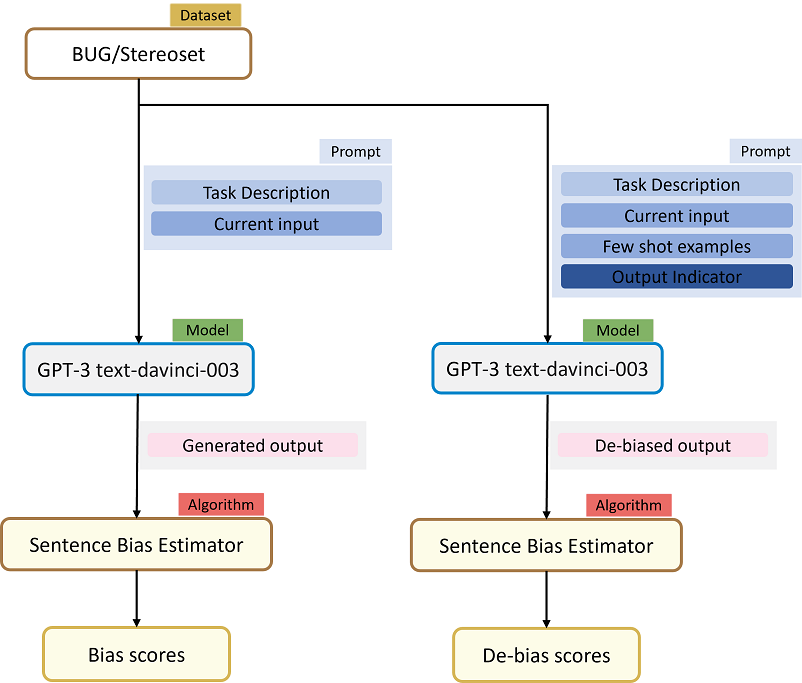
\includegraphics[width=1\linewidth]{debias.png}
  \caption{Bias Reduction Flow using GPT-3}
  \label{fig:debiasflow}
\end{figure}


\subsection{Datasets}
We are using the Balanced Bug \citep{levy2021collecting:21} and StereoSet \citep{nadeem-etal-2021-stereoset:21} data sets for our experiments.

The Balanced BUG (BB)\footnote{\url{https://github.com/SLAB-NLP/BUG}} dataset provides 25,504 sentences, balanced between male and female entities and between stereotypical and non-stereotypical gender role assignments. We use the anti-stereotypical entry as our one shot example.

The StereoSet (SS)\footnote{\url{https://github.com/moinnadeem/StereoSet}} dataset was crowdsourced and developed to evaluate bias across intrasentence and intersentence context association tests, and it consists of 4 domains (gender,
profession, race and religion), 321 target words, and 16,995 test triplets.  Each triplet consists of a context and three options representing a stereotype, anti-stereotype, and a meaningless context for each  target word and domain. We used anti-stereotype and unrelated statements from the gender domain as part of our data set for use in reducing bias in few shot learning.

\citealt{blodgett-etal-2021-stereotyping:21} have raised concerns around the validity of using data sets such as StereoSet or Wino-bias and opened the door to evaluate other datasets due to shortcomings in representing a harmful or pertinent bias. Here, we are not considering the degree of harm of the presented bias statements in evaluating their bias measurement or stereotype relevance.


\subsection{Models}

We primarily focused on using InferSent for sentence encoding in creating our bias scorer and experimenting with BERT and GPT-3.

\textbf{InferSent} is a sentence encoder trained on the Stanford Natural Language Inference dataset \citep{conneau-EtAl:17} that we use to visualize and identify the relative importance of each word to the sentence in order to generate a sentence level gender bias score.

For our experiment, we use the 'bert-large-uncased-whole-word-masking' model\footnote{\url{huggingface.co/bert-large-uncased-whole-word-masking}} as our MLM and GPT-3 text-davinci-003 model\footnote{\url{https://beta.openai.com/docs/models/gpt-3}} as our ALM. As part of our initial review process, we also ran experiments using the models listed in \autoref{tab:hostedmodels} related to sentence-similarity, entailment, fill-mask, question-answer, zero-shot-classification tasks invoked by the classes in our framework shown in \autoref{fig:explainerclasses}. We selected BERT and GPT-3 for our primary model experimentation to demonstrate the progression from BERT as the previous state of the art PLM and to investigate the gender bias performance of the recently released Davinci-003 model. 

\section{Results and discussion}

\subsection{Ablations}

\textbf{Bias Estimation for BERT and GPT-3 at the Sentence Level}

We visualize one example of a  sentence's individual word embeddings and their relative contribution to the sentence (\autoref{fig:sentencewordimpt}) as well as the individual gender bias score of each word embedding (\autoref{fig:world-level-bias}) as inputs to generate a final bias sentence level score. 

When using the same masked example 'They said that John really wanted a [MASK] for his birthday', the sentence's fine Weighted gender bias was lower for GPT-3 than BERT for this coreference task, and in general ALMs perform better than MLMs. The results can be reviewed under \autoref{fig:gpt3sentencebias} and \autoref{fig:bertsentencebias}.

When we prompt with GPT-3 to 'Replace [MASK] and return sentence' with a 2-shot set of human created examples of 'John likes to play with flowers' and ''John like to play with Ribbons', we attain a further reduction in the fine weighted gender bias of -1.88930 \autoref{fig:gpt3exfewshot}. As the sentence fine bias score approaches zero, the gender bias for the sentence reduces.

\textbf{Comparison between BERT, Zero Shot GPT-3, and Few Shot GPT-3}

Using this framework, we ran through the Balanced BUG (BB) and StereoSet (SS) data sets using both the BERT and GPT-3 models. For one shot learning, BB was used and for few shot learning SS was used. \autoref{fig:avg-bias-scores} shows a rolling average of the bias scores for GPT-3, GPT-3 few shot and BERT models. We can observe that the GPT-3 Few shot method produces fewer biased words and is better for sentences containing more gender biased words (bias score >12.5). \autoref{fig:bias-trend-plot} shows that overall, few shot learning delivers a better bias score especially when sentences contain stronger biased words.

\begin{figure}
  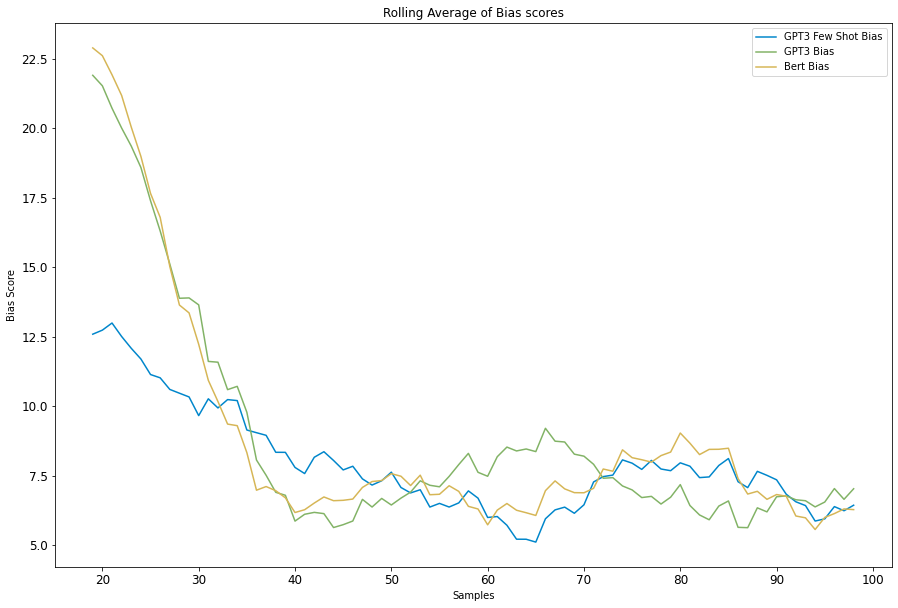
\includegraphics[width=1\linewidth]{img/avg-bias-scores.png}
  \caption{Line plot shows the distribution of samples by bias scoring by model.}
  \label{fig:avg-bias-scores}
\end{figure}

\textbf{Self-Instructed Prompt Generation using GPT-3 Davinci-003}

\citealp[in their paper \emph{Self-diagnosis and self-debiasing: A proposal for reducing corpus-based bias in nlp}]{schick2021self:21} also leveraged PLM output into their framework. They show that PLMs can recognize sentences as being biased based on the presence of particular keywords. However their work preceeds recent advances in ALMs and few-shot based instructions. Their framework mostly endeavors to prevent models from generating banned words, rather than working at higher levels of NLU and emergent abilities of large language models (LLMs). We ask LLMs to create multiple gender-debiased sentences and instruct the LLM to generate text in a similar style with the few shot assembly. This forces the LLM to work within the context of sentence similarity and textual style \citep{suzgun2022prompt:22}. Appendix \ref{appendix:self instruction pipeline} provides examples of \emph{self-instruct}.
\subsection{Discussion}
We walk through the respective improvement in bias reduction from word embedding, MLM, and zero shot prompting to show that few shot learning with prompting can successfully reduce gender bias extrinsic to the model pretraining and without the use of fine tuning.

While GPT-3 shows significant improvement in core model capabilities, zero shot output does not show similar advances in gender debiasing. This reinforces the role of few shot learning in not only GPT-3 but also for new PLMs.

\subsection{Limitations}

One limitation in our exploration includes the distinction between debiasing and gender bias reduction. In using anti-stereotypical and neutral statements, we reduce the overall bias score for sentences, but this does not necessarily debias the sentence embeddings as the score can be changed to the opposite geometry direction in the vector space. Additionally, only two genders are considered.

Not having a ready-made few shot gender bias data set was challenging for our baseline exploration, we had to resort to anti-stereotypes to calibrate the bias, although this worked, we believe that having more directed few shot examples for the inputs would have produced better results. 

Use of the latest GPT-3 text-davinci-003 model incurred financial costs that limited the scope of exploration and the number of samples that were evaluated in the experiments.

\section{Conclusion}
We describe gender bias at a word embedding and contextual sentence level within PLMs and present the role of few shot learning in prompt engineering tasks as a viable method to reduce gender bias. 

We evaluate few shot learning with the newly released GPT-3 DaVinci-003 and show that few shot learning successfully reduces gender bias below that of zero shot outputs.

We explored self-instruction by generating prompts / few shot examples by prompting the PLM to reduce gender bias.

Understanding how to identify harmful bias and how to measure and reduce gender and other forms of bias remains unsolved and continues to be an active area of NLP research. Few shot learning has a role in prompt engineering LLMs that are new, have limited bias evaluation by researchers, or for models that have cost or computational constraints. 

In considering future research, we would increase our sample size, further study the differences between fine tuning compared to few shot performance for  self-generated few shot examples as well as explore  synthetic generation of a bias data set for few shot prompt input learning by self-administered debiasing through ALM self-generated prompting. We envision LLM's will automate more sections of the gender reduction pipeline within text-generation tasks. Just as LLMs can generate images based on visual style prompts, we anticipate text-generation will adapt writing styles. 


\section{Acknowledgments}
We would like to thank Jennifer Zhu, Natalie Ahn, Mark Butler, and the W266 instruction team who supplied feedback and guided the direction of the paper. We acknowledge the OpenAI GPT-3 DaVinci-003 model for its contribution in generating this paper's title.

\bibliography{acl_latex}
% Set single column format for appendices

\onecolumn
\begin{appendices}

% Self-Instruction: \ref{appendix:self-instruction} such as \ref{appendix:self-instruction}

\section{Self-Instruction}\label{appendix:self instruction pipeline}

\citealp{meade_2022_empirical:22} benchmarked different debias frameworks using StereoSet and Crows\_Pairs and concluded that self\textendash debias \citep{schick2021self:21} was the most effective framework. The authors contributed Bias-Bench\footnote{\url{https://github.com/mcgill-nlp/bias-bench}} as part of their paper. We approach the problem in a similar fashion, where PLMs play an active role in prompt assembly. We detail the \textbf{self-instruct} prompt assembly that uses our framework that calls either HuggingFace or OpenAI inference APIs. As show in Figure \ref{fig:nongenderbiasedstatements}, within a jupyter notebook, we ask the ALM (davinci-003) for non-gender-biased-statements and retrieve its answer within a pandas DataFrame. Similar to HuggingFace's Pipelines, our API returns a class that specializes in the functionality attached to the \emph{instruction} task. Our framework has a similar API that creates tasks to input prompts and retrieve PLM prompt completion output for sentence-similarity, question-answer, instructions, zero-shot-classification, entailment-classification and embeddings. 

\begin{figure}[H]
  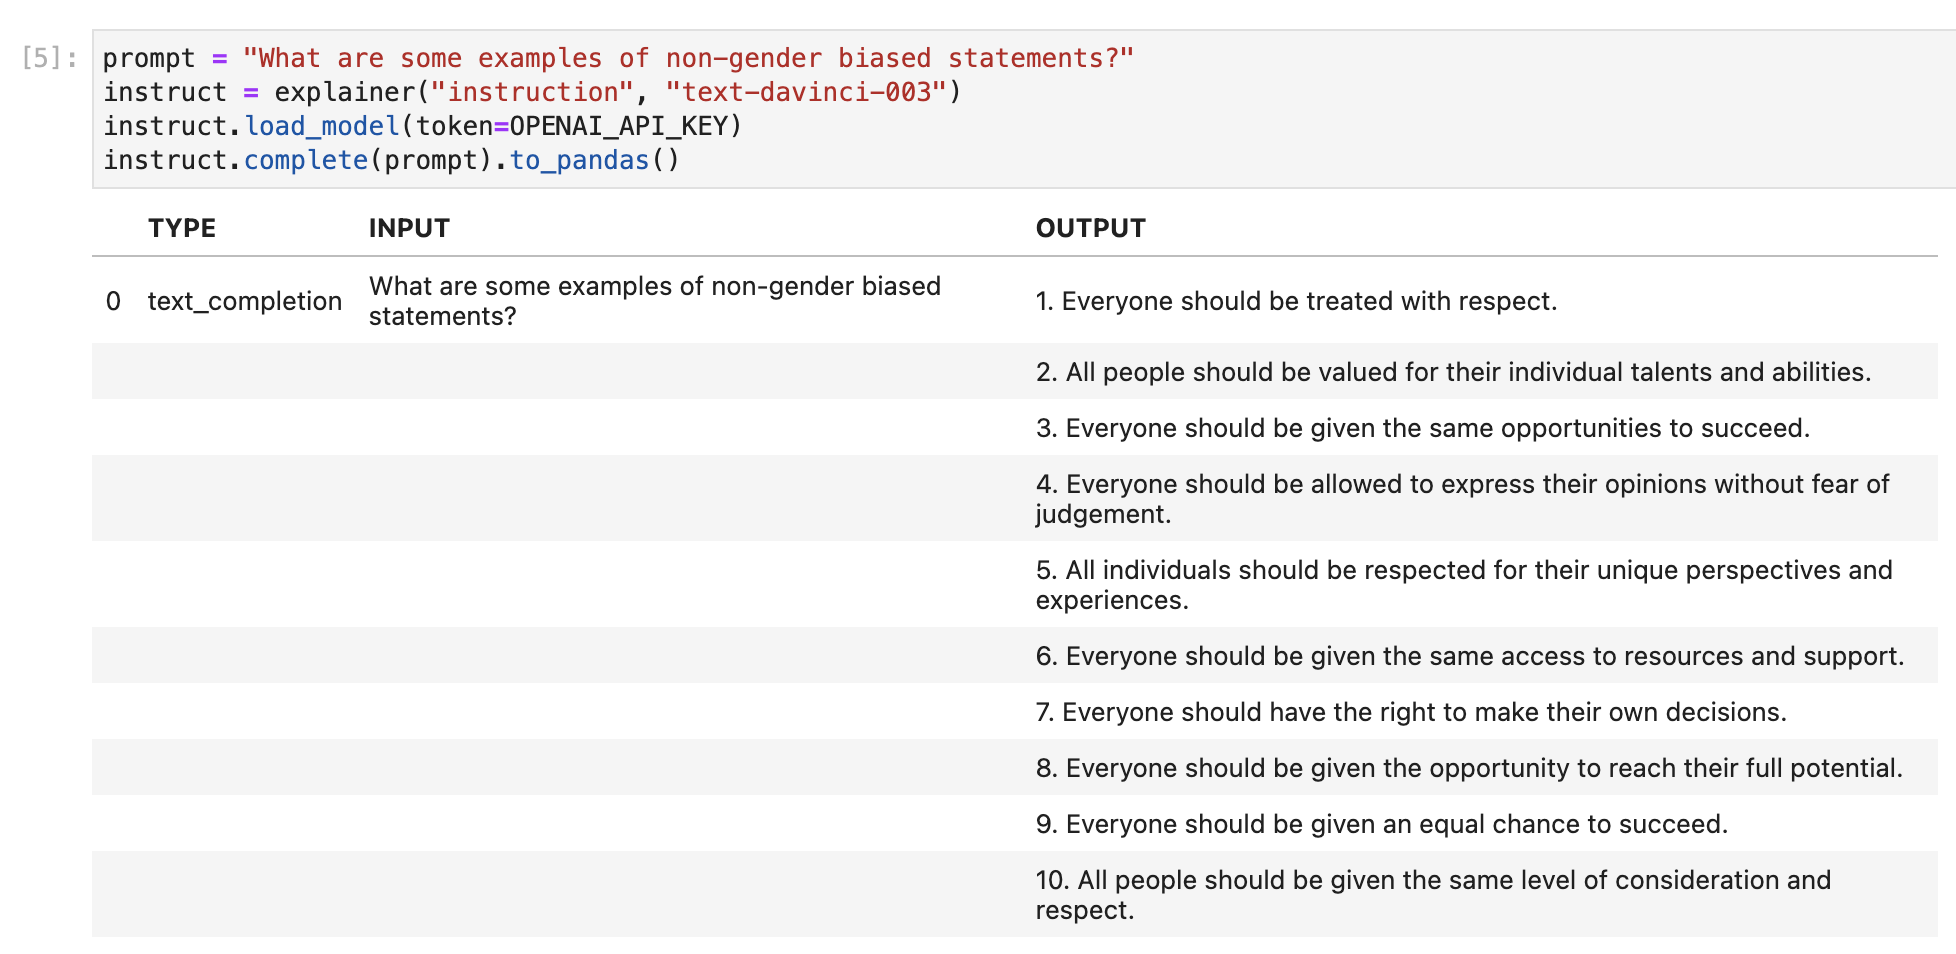
\includegraphics[width=\linewidth]{img/non-gender-biased-statements.png}
  \caption{Retrieving non-gender-biased statements from davinci-003}
  \label{fig:nongenderbiasedstatements}
\end{figure}

\begin{figure}[H]
  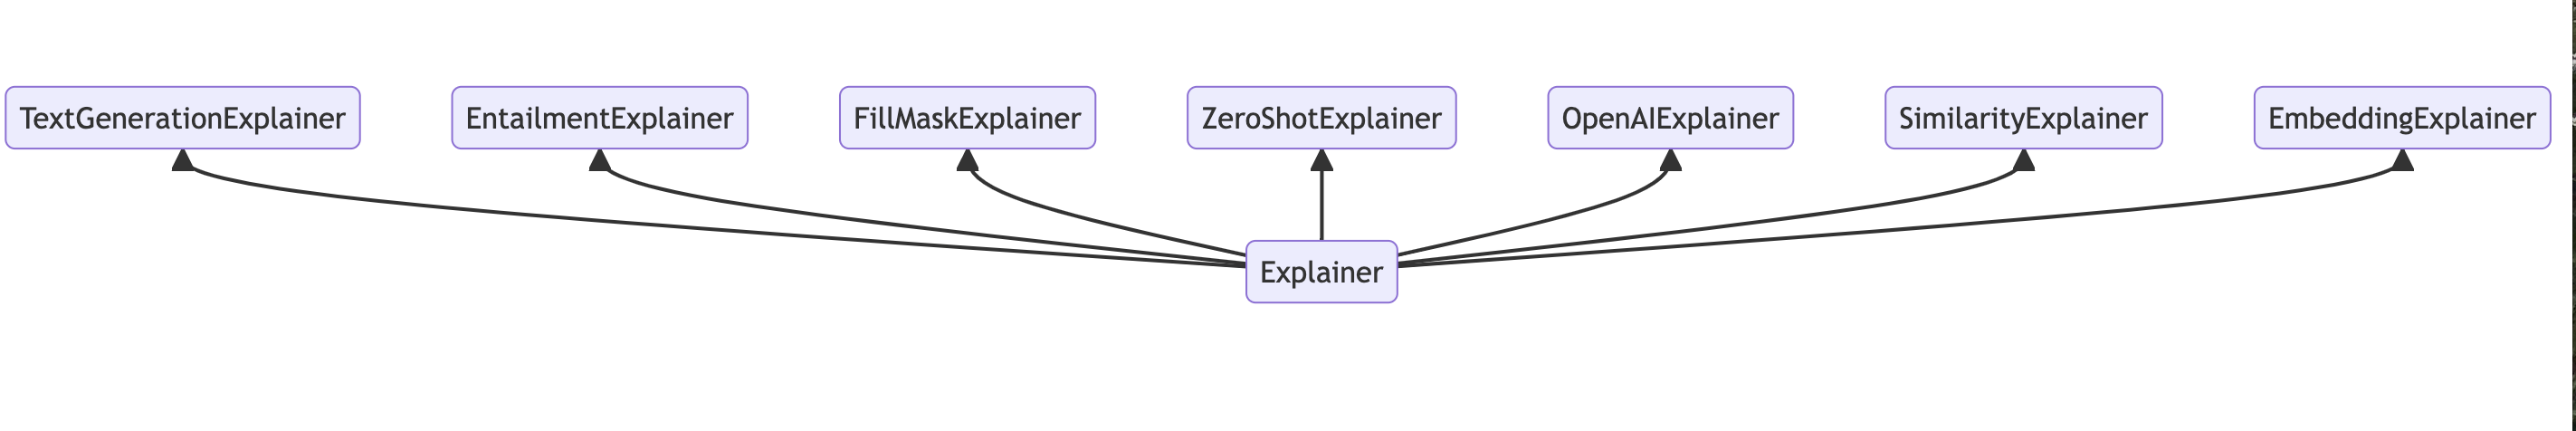
\includegraphics[width=\linewidth]{img/explainerinheritance.png}
  \caption{Explainer Classes}
  \label{fig:explainerclasses}
\end{figure}

  

\section{Cross Reference Tables and Figures}\label{appendix:crossreferences}

\begin{table}[H]
\small
\centering
\begin{tabular}{l|l}
\hline
\textbf{Github} & \textbf{Reference}\\\hline
\url{https://github.com/tolga-b/debiaswe} & \citealt{bolukbasi2016man:16}\\
\url{https://github.com/pliang279/LM\_bias} & \citealt{liang2021towards:21}\\ 
\url{https://github.com/12kleingordon34/NLP} & \citealt{de2021stereotype:21}\\ 
\url{https://github.com/FEE-Fair-Embedding-Engine/FEE} & \citealt{kumar2020fair:20}\\ 
\url{https://github.com/princeton-nlp/MABEL} & \citealt{he2022mabel:22}\\
\url{https://github.com/iPieter/biased-rulers} & \citealt{delobelle2022measuring:22}\\
\url{https://github.com/oxai/debias-vision-lang} & \citealt{berg2022prompt:22}\\
\url{https://github.com/wolferobert3/gender\_bias\_swe\_aies2022} & \citealt{caliskan2022gender:22}\\
\hline
\end{tabular}
\caption{Debias framworks on Github}
\label{tab:debiasimpl}
\end{table}

\begin{table}[H]
\centering
\begin{tabular}{l|l}
\hline
\textbf{Model} & \textbf{Resource}\\\hline
BigScience T0 \citep{sanh2021multitask:21} & \url{https://github.com/bigscience-workshop/t-zero}\\
BIG-bench \citep{srivastava2022beyond:22} & \url{https://github.com/google/BIG-bench/tree/main/}\\
PromptSource \citep{bach2022promptsource:22} & \url{https://github.com/bigscience-workshop/promptsource/}\\
OpenPrompt \citep{ding2021openprompt:22} & \url{https://github.com/thunlp/OpenPrompt.git}\\
\hline
\end{tabular}
\caption{Prompt Hubs}
\label{tab:prompthubs}
\end{table}

\begin{table}[H]
\centering
\begin{tabular}{l|l}
\hline
\textbf{Model} & \textbf{Paper}\\\hline
bart\textendash large\textendash mnli\tablefootnote{\url{https://huggingface.co/facebook/bart-large-mnli}} & \citealp{yin2019benchmarking:19}\\
T0\_B3\tablefootnote{\url{https://huggingface.co/bigscience/T0_3B}} & \citealp{sanh2021multitask:21}\\
stsb\textendash xlm\textendash r\textendash multilingual\tablefootnote{\url{https://https://huggingface.co/sentence-transformers/stsb-xlm-r-multilingual}} & \citealp{reimers-2019-sentence-bert:19}\\
gpt\textendash j\textendash 6B\tablefootnote{\url{https://huggingface.co/EleutherAI/gpt-j-6B}} & \citealp{gpt-j:21}\\
\hline
\end{tabular}
\caption{Hosted Models (HuggingFace and OpenAI)}
\label{tab:hostedmodels}
\end{table}

\begin{table}[H]
\centering
\begin{tabular}{l|l}
\hline
\textbf{Dataset} & \textbf{Reference}\\\hline
P3\tablefootnote{\url{https://huggingface.co/datasets/bigscience/P3}} & \citealt{sanh2021multitask:21}\\
\hline
\end{tabular}
\caption{Huggingface Hosted Datasets}
\label{tab:huggingfacedatasets}
\end{table}

\begin{table}[H]
\small
\centering
\begin{tabular}{l|l}
\hline
\textbf{Github} & \textbf{Reference}\\\hline
\url{https://github.com/beir-cellar/beir} & BEIR \citep{thakur2021beir:21}\\
MISSING & \citep{yin2019benchmarking:19}\\
\hline
\end{tabular}
\caption{Zero and Few-Shot Benchmarks on Github}
\label{tab:zero-fewshot-benchmarks}
\end{table}

\begin{table*}
\small
\centering
\begin{tabular}{l|l}
\hline
\textbf{Github} & \textbf{Reference}\\\hline
\url{https://github.com/facebookresearch/ELECTRA-Fewshot-Learning} & ELECTRA \citep{xia2022prompting:22}\\
\url{https://github.com/princeton-nlp/LM-BFF} & LM\textendash BFF \citep{gao2020making:20}\\
\url{https://github.com/dapascual/K2T} & Keyword2Text \citep{pascual2021plug:21}\\
TDB & ADEPT \citep{yang2022adept:22}\\
\hline
\end{tabular}
\caption{Zero and Few-Shot Frameworks on Github}
\label{tab:debiasimpl}
\end{table*}

Table \ref{tab:debiasimpl} lists noteworthy debiasing papers and frameworks. Table \ref{tab:huggingfacedatasets} lists datasets referenced in this paper. Table \ref{tab:hostedmodels} shows the models hosted on huggingface, along with the parameter sizes. 



%\setcounter{figure}{0}    
\begin{figure}[H]
  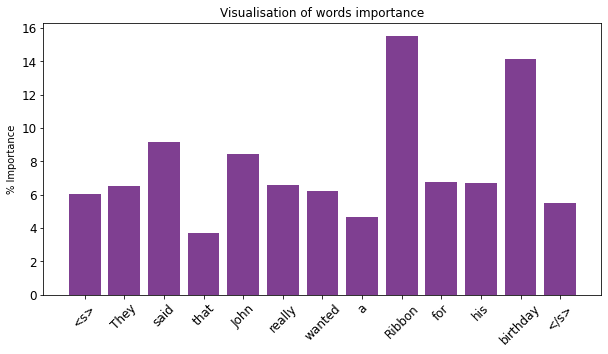
\includegraphics[width=\linewidth]{img/sentence-word-impt.png}
  \caption{Graph shows the relative importance of each word to the sentence meaning after being processed through the InferSent sentence encoder.}
  \label{fig:sentencewordimpt}
\end{figure}

\begin{figure}[H]
  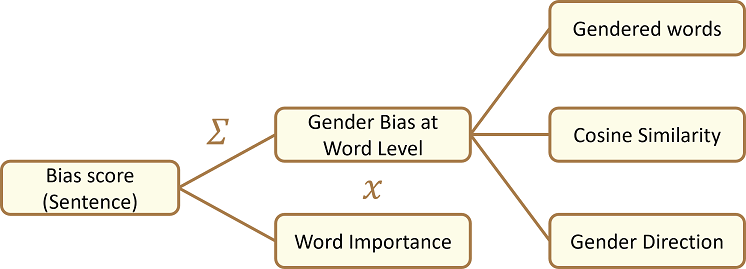
\includegraphics[width=\linewidth]{sentence-bias-score.png}
  \caption{Sentence Bias Score Process Flow}
  \label{fig:sentencescore}
\end{figure}

\begin{figure}[H]
  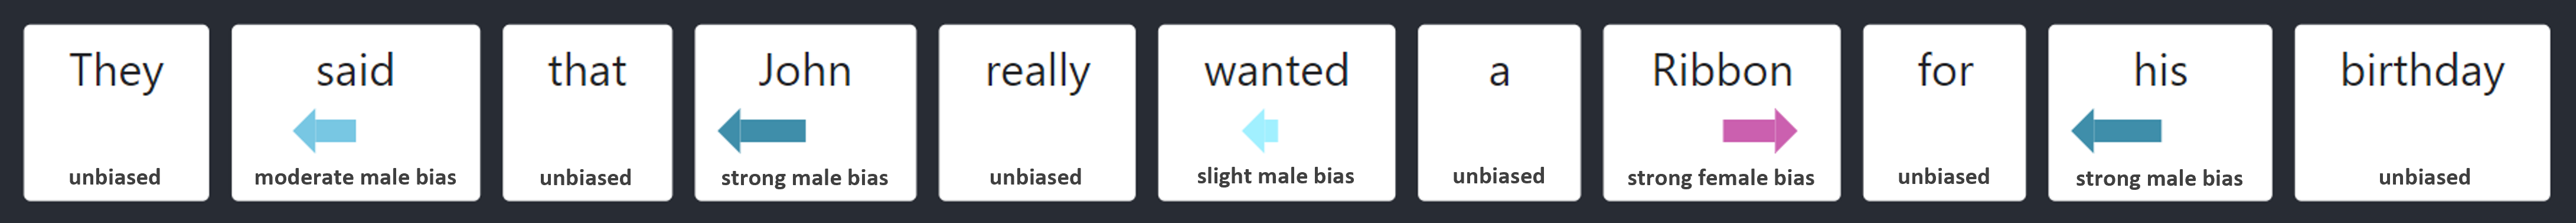
\includegraphics[width=\linewidth]{img/word-level-bias.png}
  \caption{Word Vector Embedding Gender Bias Representation}
  \label{fig:world-level-bias}
\end{figure}

\begin{figure}
  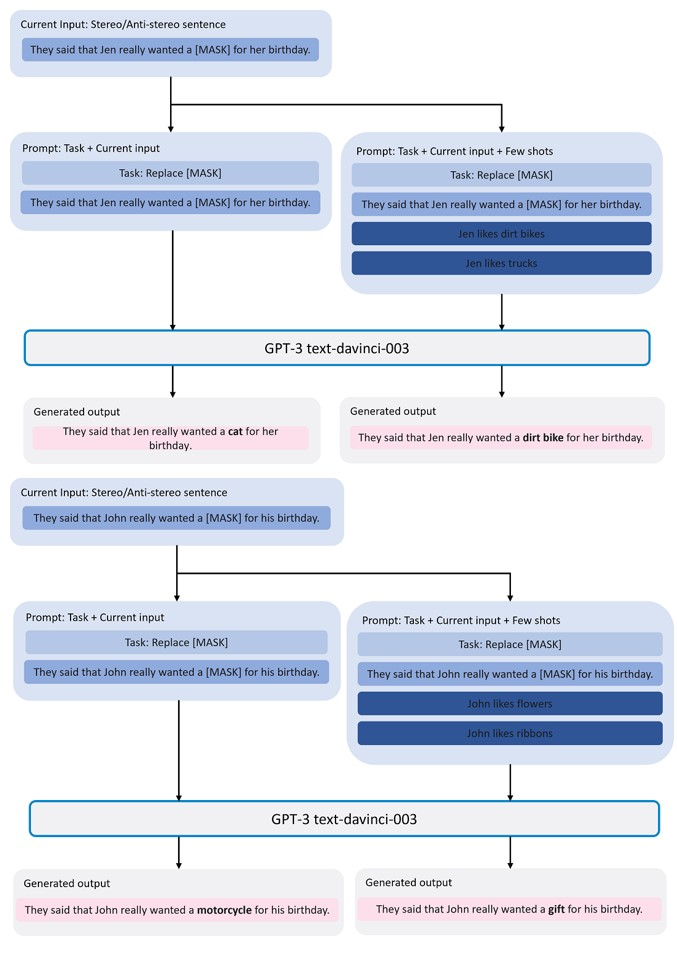
\includegraphics[width=\linewidth]{fewshotprompt.jpg}
  \caption{Few shot prompt with GPT-3}
  \label{fig:fewshotprompt}
\end{figure}

\begin{figure}
  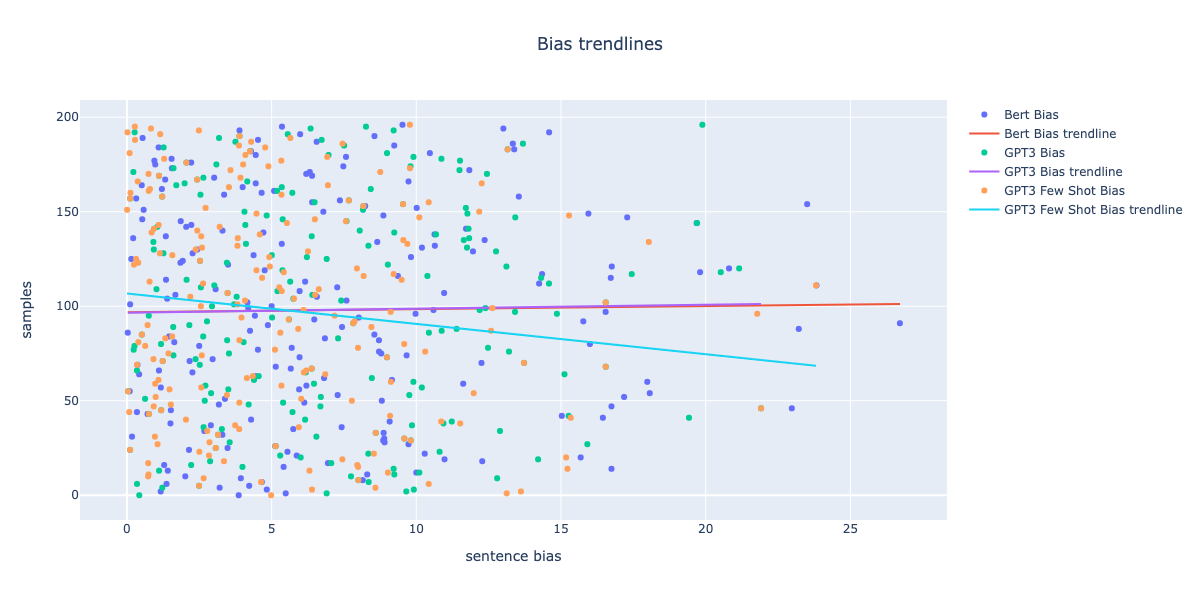
\includegraphics[width=\linewidth]{img/bias-trend-plot.png}
  \caption{Line plot shows the distribution of samples by bias scoring by model.}
  \label{fig:bias-trend-plot}
\end{figure}

\begin{figure}
  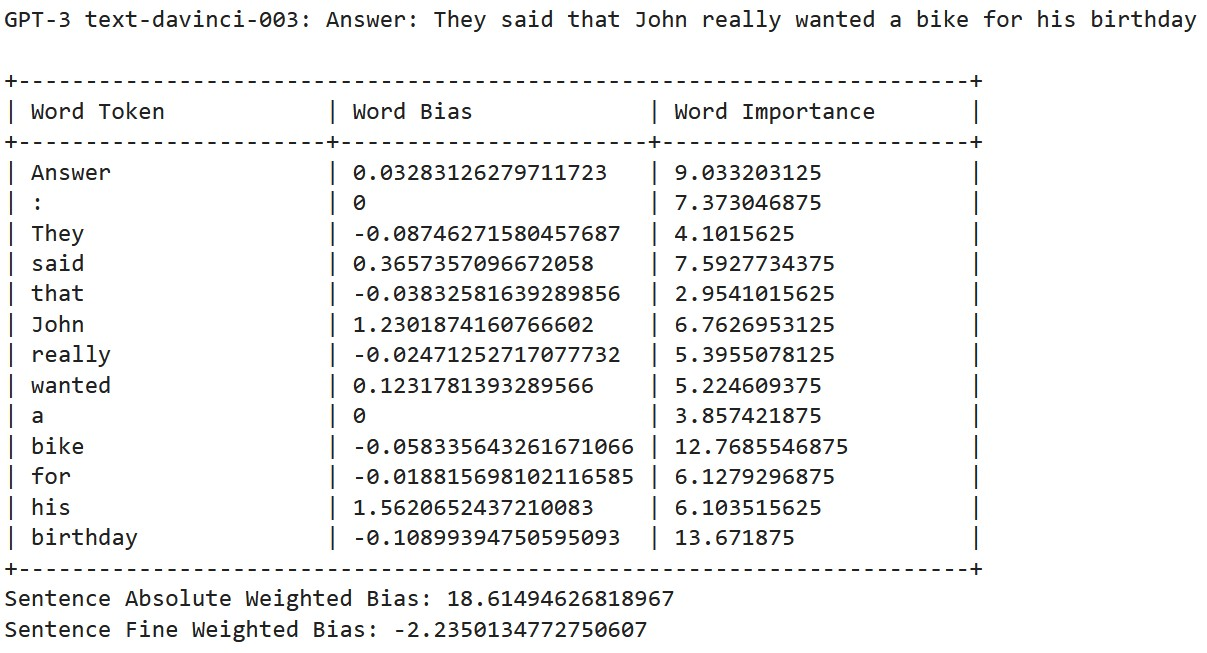
\includegraphics[width=\linewidth]{img/gpt3sentencebias.jpg}
  \caption{Sentence bias for example sentence using GPT3.}
  \label{fig:gpt3sentencebias}
\end{figure}

\begin{figure}
  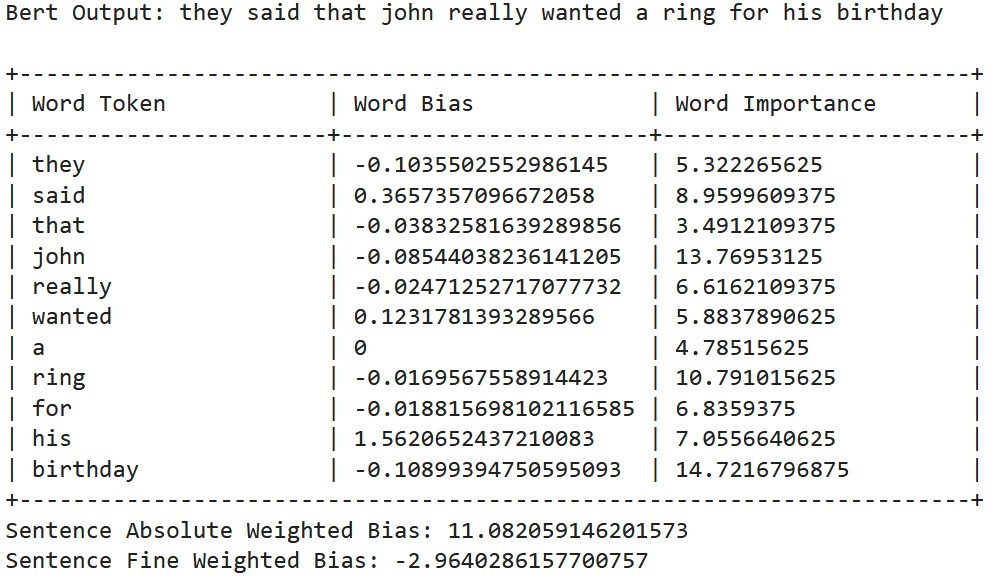
\includegraphics[width=\linewidth]{img/bertsentencebias.jpg}
  \caption{Sentence bias for example sentence using BERT.}
  \label{fig:bertsentencebias}
\end{figure}

\begin{figure}
  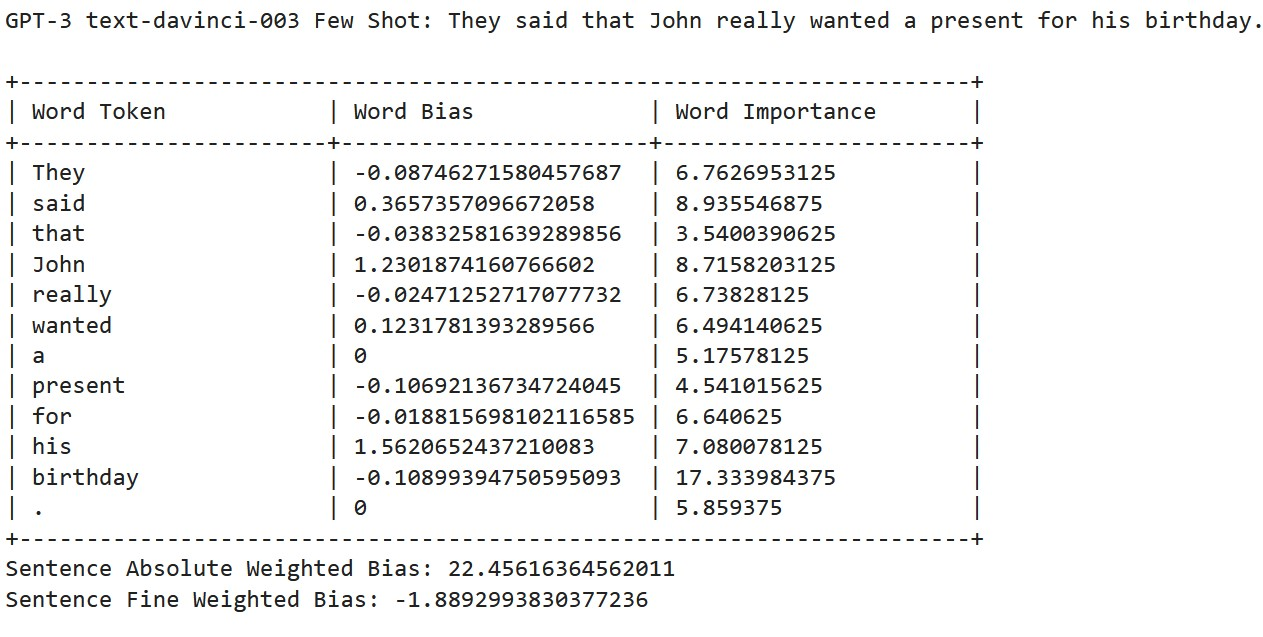
\includegraphics[width=\linewidth]{img/gpt3exfewshot.jpg}
  \caption{Sentence bias for example sentence using few shot learning with GPT-3.}
  \label{fig:gpt3exfewshot}
\end{figure}

\end{appendices}

\end{document}
